\documentclass{ximera}

\newcommand{\RR}{\mathbb R}
\renewcommand{\d}{\,d}
\newcommand{\dd}[2][]{\frac{d #1}{d #2}}
\renewcommand{\l}{\ell}
\newcommand{\ddx}{\frac{d}{dx}}
\newcommand{\dfn}{\textbf}
\newcommand{\eval}[1]{\bigg[ #1 \bigg]}


\author{Bart Snapp}

\outcome{Estimate line integrals.}

\begin{document}
\begin{exercise}
  Let $\vec{F}:\R^2\to\R^2$ be roughly described by the following
  table of values:
  \begin{image}
    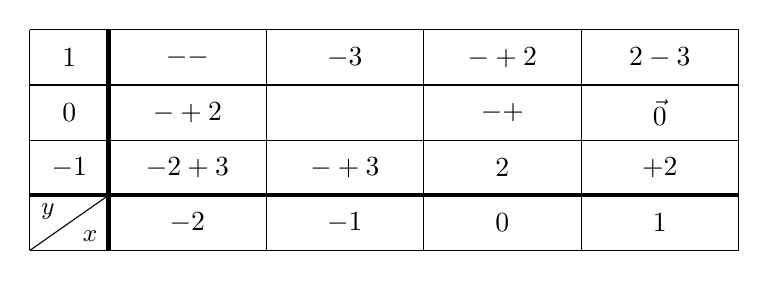
\begin{tikzpicture}[x=1cm,y=.7cm]
      
      
      \draw (0,0) grid [step=1] (1,4);
      \draw (3,4) -- (3,0);
      \draw (5,4) -- (5,0);
      \draw (7,4) -- (7,0);
      \draw (9,4) -- (9,0);
      
      \draw (0,0) -- (9,0);
      \draw (0,1) -- (9,1);
      \draw (0,2) -- (9,2);
      \draw (0,3) -- (9,3);
      \draw (0,4) -- (9,4);
      

      
      \draw[ultra thick] (0,1)--(9,1);
      \draw[ultra thick] (1,4)--(1,0);
      
      \draw (0,0) -- (1,1);
      %\node at (.9,.9) [below left,inner sep=1pt] {\small$y$};
      %\node at (0.1,.1) [above right,inner sep=1pt] {\small$x$};
      \node at (.1,.9) [below right,inner sep=1pt] {\small$y$};
      \node at (0.9,.1) [above left,inner sep=1pt] {\small$x$};
      
      
      %% x-values
      \node at (2,.5) {$-2$};
      \node at (4,.5) {$-1$};
      \node at (6,.5) {$0$};
      \node at (8,.5) {$1$};
      
      %% y-values
      \node at (0.5,1.5) {$-1$};
      \node at (0.5,2.5) {$0$};
      \node at (0.5,3.5) {$1$};
      
      
      %% vectors
      %% bottom row
      \node at (2,1.5) {$-2\veci+3\vecj$};
      \node at (4,1.5) {$-\veci+3\vecj$};
      \node at (6,1.5) {$2\vecj$};
      \node at (8,1.5) {$\veci+2\vecj$};
      
      %% second row
      \node at (2,2.5) {$-\veci+2\vecj$};
      \node at (4,2.5) {$\vecj$};
      \node at (6,2.5) {$-\veci+\vecj$};
      \node at (8,2.5) {$\vec{0}$};
      
      %% third row
      \node at (2,3.5) {$-\veci-\vecj$};
      \node at (4,3.5) {$\veci-3\vecj$};
      \node at (6,3.5) {$-\veci+2\vecj$};
      \node at (8,3.5) {$2\veci-3\vecj$};
      
    \end{tikzpicture}
  \end{image}
  Let $\vec{p}(t)$ be the vector-valued function describing the line
  $\l$ running from the point $(1,-1)$ to $(-1,1)$ as $t$ runs from
  $0$ to $1$. Setting $\d t = 1/3$, estimate:
  \[
  \int_\l \vec{F}\dotp\d\vec{p}
  \]
  \begin{prompt}
    \[
    \vec{p}(t) = \vector{\answer{1-2t},\answer{-1+2t}}
    \]
    \[
    \int_\l \vec{F}\dotp\d\vec{p} \approx\answer{-2/3}
    \]
  \end{prompt}
\end{exercise}
\end{document}
